\lecture{2}{22 Jan. 10:00}{Newton's Second Law}
\subsection{Newton's Second Law}
Here we present a different formulation of Newton's Second Law than A-levels.

\begin{definition}{}{}
    The \textit{equation of motion} of a particle subjected to a force \(\mathbf{F} \) is
    \[
        \frac{\mathrm{d}}{\mathrm{d}t} (m \dot{\mathbf{x}}) = \mathbf{F} (\mathbf{x}, \dot{\mathbf{x}})
    \]
    where \(\mathbf{p} = m \dot{\mathbf{x}}\) is \textit{momentum}, \(m\) is \textit{inertial mass}, It is a measure of the reluctance of a particle to move.
\end{definition}

When \(\frac{\mathrm{d}m}{\mathrm{d}t} = 0\) (so true in most situations), we have
\begin{theorem}{Newton's Second Law}{}
    \[
        m\ddot{\mathbf{x}} = \mathbf{F} (\mathbf{x}, \dot{\mathbf{x}}).
    \]
\end{theorem}
The equation above of motion is a second order differential equation, so we need to specify two initial conditions for each degree of freedom.

\begin{example}
    When \(\mathbf{x} \in \mathbb{R}^3\), we have three degrees of freedom, so we need six initial conditions. 
\end{example}

There are two steps in any Newtonian mechanics problem:
\begin{itemize}
    \item Write down the equations(s),
    \item Solve it.
\end{itemize}

\section{Forces}
\subsection{Potentials in One Dimension}
Consider a particle moving in a line with position \(x(t)\). Suppose that \(F = F(x)\), i.e. it depends on position, not on velocity. We define a \textit{potential energy} \(V(x)\) by
\[
    F = -\frac{\mathrm{d}V}{\mathrm{d}x} \quad \text{x} \quad V(x) = - \int_{x_0}^{x}\mathrm{d}x'F(x').
\]
Note that the prime does not denote derivative here; \(x'\) is a dummy variable.

The equation of motion is
\begin{equation}
    m\ddot{x} = -\frac{\mathrm{d}V}{\mathrm{d}x}.
    \label{1dmo}
\end{equation}

\begin{proposition}{}{}
    The energy \(E = \frac{1}{2}m\ddot{x}+V(x)\) is conserved (i.e. \(\dot{E} = 0\)) for any trajectory which obeys the equation of motion.
\end{proposition}
\begin{proof}
    We have the following,
    \begin{align*}
        \frac{\mathrm{d}E}{\mathrm{d}t} &= m\dot{x}\ddot{x} + \frac{\mathrm{d}V}{\mathrm{d}x} \dot{x}\\
        &=\dot{x}(m\ddot{x} + \frac{\mathrm{d}V}{\mathrm{d}x})\\
        &=0\quad \text{by \eqref{1dmo}}
    \end{align*}
\end{proof}
Note, however, if \(F = F(x, \dot{x})\), there is no conserved quantity.

\begin{example}[Harmonic Oscillater]
    When \(V = \frac{1}{2}kx^2\), \eqref{1dmo} becomes \(m\ddot{x}] = -kx\). And the general solution is
    \[
        x(t) = A\cos(wt) + B\sin(wt)
    \]
    where \(w\coloneqq \sqrt{\frac{k}{m}}\) is the \textit{angular frequency}. \(A\) and \(B\) are integration constants.

    It's simple to show that \(E = \frac{1}{2}m\dot{x}^2 +\frac{1}{2}kx^2\) is constant.

    The time taken to complete a cycle is the \textit{period} \(T = \frac{2\pi}{\omega}\).
\end{example}

For a general potential \(V(x)\), the conserved quantity allows us to solve any one-dimensional problem.
\begin{align*}
    E &= \frac{1}{2} m\dot{x}^2 + V(x)\\
    \implies \frac{\mathrm{d}x}{\mathrm{d}t} &= \pm \sqrt{\frac{2}{m}(E - V(x))}\\
    \implies t - t_0 &= \pm \int_{x_0}^x \frac{dx'}{\sqrt{\frac{2}{m}(E - V(x'))} }
\end{align*}
which is the solution, and we just need to do the integral.

\subsection*{Motion in a Potential}
Sometimes even if you can't do the integral, it's simple to get a qualitative picture of the solution.
\begin{example}
   If the potential is \(V(x) = m(x^3 - 3x)\).
   \begin{figure}[h]
       \centering
       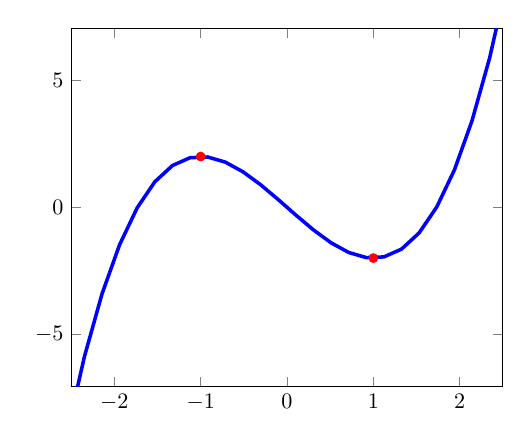
\begin{tikzpicture}[scale=0.8]
        \begin{axis}[xmin=-2.5,xmax=2.5, samples=50]
          \addplot[blue, ultra thick] (x,x^3-3*x);
          \addplot [red, mark=*] coordinates {(-1, 2)};
          \addplot [red, mark=*] coordinates {(1, -2)};
        \end{axis}
        \end{tikzpicture}
       \caption{Graph of the potential function}
       \label{fig:pot}
   \end{figure}
   If we drop the particle at \(x = x_0\), the total energy \(E = V(x_0)\) which is all potential. We have the following several cases,
   \begin{enumerate}
       \item \(x_0 = \pm 1\implies\) particle stays there at all time because \eqref{1dmo} says there must be no force.
       \item \(x_0 \in (-1,2)\implies\) particle oscillates back and force in dip.

       The initial energy is all potential, and it turns this into kinetic energy and falls down the dip.
   \end{enumerate}
\end{example}